\chapter{Código implementado}

\section{Classes Auxiliares}

As classes criadas são as seguintes:

\begin{itemize}
    \item \textit{\textbf{Accuracy}} - Classe responsável por armazenar a informação sobre as trajetórias inimigas.
    
    Supondo o normal funcionamento da equipa, os robots \textit{Destroyers} são os únicos a realizar ataques à equipa inimiga. 
    Para desempenhar esta tarefa, os \textit{Destroyers} recebem ordens para atacar um determinado inimigo, escolhendo 1 de 3 métodos implementados para o cálculo da trajetória de disparo. 

    À medida que o jogo se desenvolve, são guardados registos de cada disparo de forma a que, num disparo futuro, se observe a média de \textit{accuracy} que cada algoritmo obtém num determinado contexto com o robot inimigo.  
    Cada método/algoritmo de previsão de movimentos/trajetória assume três cenários: o inimigo pode deslocar-se linearmente, em círculos ou estar imóvel, num estado estacionário.
    
    
    \item \textit{\textbf{CircularIntercept}} - Esta classe invoca métodos que realizam a atualização da previsão da posição de um robot inimigo. 
    
    A classe estende a classe \textit{Intecept} e, tal como o nome indica, é utilizada para definir que a previsão da posição do robot inimigo assume um movimento circular do mesmo, em vez de um movimento linear. 
    
    Assim, para calcular qual a direção sobre a qual realizar um disparo, assume-se que o inimigo está a deslocar-se num percurso circular. 
    
    \item \textit{\textbf{Coordinate}} - Classe criada para representar um ponto com coordenadas X,Y. 
    
    Estas coordenadas são posteriormente utilizadas para identificar objetos, pontos a evitar ou inimigos dentro das dimensões do campo de batalha. 
    
    \item \textit{\textbf{Gravity}} - Classe utilizada para implementar o algoritmo de \textit{Anti-Gravity Movement}. 
    
    A tática implementada nesta classe permite calcular as trajetórias que cada robot deve seguir ao longo do decorrer de uma \textit{round} de um jogo;
    
    \item \textit{\textbf{Intercept}} - Classe responsável por calcular a previsão das próximas coordenadas de um robot.
    
    Para isso, os métodos têm por base a posição inicial/atual do robot, a sua direção e a velocidade, selecionando um possível tipo de trajetória (movimento linear, circular ou estacionário), calcula com os parâmetros citados a nova posição do robot;
    
    \item \textit{\textbf{Order}} - Implementação que representa uma ordem/instrução enviada do \textit{Seeker} para os \textit{Destroyers}.
    
    Esta classe possui informações sobre o tipo da ordem disparar, andar, rodar, atualizar informações sobre as coordenadas para as quais disparar, coordenadas para as quais nos devemos deslocar e ângulos a rodar
    
    \item \textit{\textit{Orders}} - Classe simples que implementa uma abstração de uma lista de ordens, de forma a enviar várias ordens ao mesmo tempo aos \textit{Destroyers};
    
    \item \textit{\textbf{Point}} - Classe semelhante à \textit{Coordinate}. 
    Além de guardar as coordenadas (X,Y) de um ponto, tem também o seu "poder" de atração, de forma a implementar os conceitos da tática "Anti-Gravity". 
    
    Se o poder de atração de uma determinada coordenada for positivo é um ponto atrator, se for um ponto negativo representa um ponto repulsor. Estas coordenadas podem representar um inimigo ou elementos da própria equipa; 
    
    \item \textit{\textbf{State}} - Estado lido a partir de um \textit{robot}, contem todas as informações lidas pelo scanner e a posição onde foi encontrado o robot em questão;
    
    \item TeamInfo - Contem o estado atual do jogo, desde pontos de gravidade, inimigos, membros da equipa e os respetivos estados e  o robot inimigo prioritário a abater;
\end{itemize}


\section{Classes Principais}

Neste projeto definimos que a nossa equipa iria ser constituída por dois tipos de robots, um deles seria o líder da equipa equipado com um radar para que possa conhecer o estado do jogo e informar o resto da equipa e o outro seria um \textit{droid}, que tem a vantagem de ter mais 20 pontos de energia, porem, não tem radar e depende de um líder para lhe indicar o que fazer.

Alem do comportamento enunciado em baixo os dois robots tem tambem alguns pontos em comum, como funções que são ativadas por eventos, como \textit{onHitWall()} e \textit{onHitByBullet()}, que nestes casos executam pequenas tarefas como mudar o seu ângulo ou movimentar se um pouco de forma a corrigir alguns comportamentos do algoritmo principal de deslocamento.

\subsection{Droid - Destroyer}

O \textit{Destroyer} é o robot com comportamento mais simples. Este aplica o algoritmo de \textit{Anti-Gravity Movement} para evitar deslocar-se pelo terreno de jogo enquanto espera por mensagens do seu líder. As mensagens podem conter o estado atual do jogo de forma a que o robot se atualize, ou uma lista de ordens a serem executadas sequencialmente, sendo que cada ordem pode consistir num disparo, num deslocamento ou mudar o ângulo do robot. 
No caso de o \textit{Seeker} ficar com 0 energia, este robot deixa de receber ordens e portanto apenas continua com o seu movimento de forma a evitar ser atingido por balas inimigas, na esperança que os restantes robots se destruam quer por passar do tempo de jogo, quer por balas enviadas pelos membros da própria equipa ou até por colisões contra outros robots e paredes.

\subsection{Lider - Seeker}
O robot Seeker tem muito em comum com o \textit{Destroyer}, usa o mesmo algoritmo para efetuar movimento, mas em vez de esperar por mensagens, este é o responsável por las enviar, assim sendo, é de máxima importância que este permaneça vivo a ronda toda. Assim sendo este robot não dispara a não ser em casos extremos, como por exemplo a restante equipa já estar toda com 0 pontos de energia e os inimigos terem mais energia do que os aliados, se estas duas condições não se reunirem simultaneamente, o robot não dispara.

Ao mesmo tempo que o robot percorre o terreno roda o seu radar 360 graus por cada ronda, sendo que sempre que avistar um robot avalia se este pertence à sua equipa ou não, atualiza o estado de jogo, envia o estado de jogo a todos os robots e além disso se confirmar que encontrou um robot da outra equipa envia também  a ordem de disparo aos \textit{Droids} para que estes tentem atingir o robot em questão.




\section{Algoritmos principais}

\subsection{Anti-Gravity Movement}
Este algoritmo é baseado na criação de pontos que vão representar forças que ao serem aplicadas no nosso robot iram fazer com que este se desloque ate outro ponto.

Os pontos são criados com base na posição dos outros robots de forma a que os outros robots exerçam uma força repulsiva no robot em questão evitando assim colisões.

Por exemplo:

\begin{figure}[H]
    \centering
    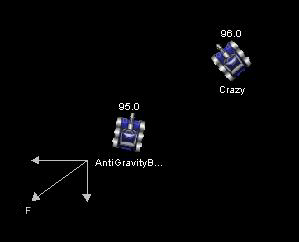
\includegraphics[scale=0.6]{Imagens/force.png}
    \caption{Esquema de forças causadas por 1 robô.}
    \label{fig:forca}
\end{figure}

Neste exemplo temos dois robots, em que o robot \textit{Crazy} executa a força F no robot \textit{AntiGravityBot}, esta força é representada por um componente em X e outro em Y.

A soma de todas as forças causadas por todos os robots irá criar a direção para a qual o robot tem de se deslocar.

Este algoritmo pode causar problemas como por exemplo, se os robots estiverem todos a direita do robot em questão, este irá ser enviado para a parede esquerda do tabuleiro e ficar preso contra a parede, para combater este problema criaram se pontos de repulsão ao longo das 4 paredes do tabuleiro desta forma combatemos o problema de ele ficar preso contra uma parede.

Alem dos pontos de repulsão criados pelas bordas e pelos robots a cada iteração deste algoritmo são definidos alguns pontos com coordenadas aleatórios, mas desta vez com forças positivas, ou seja pontos atratores, são estes pontos que iram tornar o algoritmo menos previsível e fazer com que todos os robots tenham trajetórias diferentes.

Como melhorias a este algoritmo podem ser alterados alguns parâmetros relativos as forças tais como elevar as forças a um parâmetros N e variar esse parâmetro, podemos adicionar pontos ou igualar as forças dos pontos de forma a termos um resultado mais consistente.

\subsection{Predictiv Targeting}

Para aproveitar ao máximo a energia disparada pelos robots, foi criado um método que prevê onde é que os robots irão estar nos momentos seguintes. 

Esta algoritmo tem capacidade para prever 3 situações: a primeira e mais simples é o caso do robot em questão não se mexer, ou seja se ele não se mexer a sua posição será no mesmo ponto onde foi encontrado.

Temos também um método que assume que o movimento do robot é retilíneo e uniforme e assim sendo sabendo a posição inicial do robot, a sua direção e velocidade conseguimos prever a sua próxima posição. 

Por fim, temos um terceiro método que assume que o movimento do robot é curvilíneo e tenta encontrar a posição onde o robot se irá encontrar partindo dessa assunção.

Inicialmente o robot começa por usar o algoritmo linear já que este foi considerado o caso mais comum, se este falhar testa se método de disparo para o sitio onde o robot foi encontrado e por fim, se este se mostrar pouco eficiente testa o algoritmo curvilíneo.